\documentclass{article}

% Packages
\usepackage[a4paper, margin=2.0cm]{geometry}
\usepackage{graphicx}

\usepackage{textcomp}
\usepackage{gensymb}
\usepackage{amsmath}
\usepackage{amsfonts}

\usepackage{tikz}
\usepackage{pgfplots}
\pgfplotsset{compat=newest}
\usepackage{pgfplotstable}

% Title
\title{AE2202 Fluid Dynamics - Homework 5}
\author{Hafizh Renanto Akhmad - 13621060}

\begin{document}

\maketitle

\newpage

\section*{Problem 1}
The $x$ and $y$ components of velocity for a two-dimensional flow are $u = 6y$ ft/s and $v = 3$ ft/s where $y$ is in feet. Determine the equation for the streamlines and sketch representative streamlines in the upper half plane.

\subsection*{Answer}
The streamline equation of streamline may be obtained by integrating:
\begin{equation}
    \frac{dy}{dx} = \frac{v_y}{v_x}
\end{equation}
For this case,
\begin{align*}
    \frac{dy}{dx} &= \frac{v}{u} \\
    \frac{dy}{dx} &= \frac{3}{6y} \\
    \frac{dy}{dx} &= \frac{1}{2y} \\
    2y\ dy &= dx \\
    y^2 &= x + C \\
    y^2 - x &= C
\end{align*}
Sketch:

\newpage

\section*{Problem 2}
Show that the streamlines for a flow whose velocity components are $u = c(x^2 - y^2)$ and where $v = 2cxy$, where c is a constant, are given by the equation $x^2 y - y^3 / 3 = constant$. At which point (points) is the flow parallel to the $y$ axis? At which point (points) is the fluid stationary?

\subsection*{Answer}
When the point is parallel to the $y$ axis, the velocity in $x-$direction should be zero, or:
\begin{align*}
    u &= 0 \\
    x^2 - y^2 &= 0 \\
    x^2 &= y^2 \\
    x &= \pm y
\end{align*}
Thus, the flow is parallel to the $y$ axis at $(t, \pm t)$, where $t \in \mathbb{R}$.
When the point is stationary, the velocity components are $u = 0$ and $v = 0$. 
\begin{align*}
    v &= 0 \\
    xy &= 0 \\
    x = 0\ &\vee\ y = 0
\end{align*}
Intersecting both solutions of $u = 0$ and $v = 0$, we get that the flow is stationary at $(x, y) = (0, 0)$.

\newpage

\section*{Problem 3}
The $x-$ and $y-$components of a velocity field are given by $u = (V_0 / l)x$ and $v = -(V_0 / l)y$, where $V_0$ and $l$ are constants. Plot the streamlines for this flow and determine the acceleration field.

\subsection*{Answer}
We may find the streamline equation by integrating:
\begin{equation}
    \frac{dy}{dx} = \frac{v_y}{v_x}
\end{equation}
For this case,
\begin{align*}
    \frac{dy}{dx} &= \frac{v}{u} \\
    \frac{dy}{dx} &= \frac{-(V_0 / l)y}{(V_0 / l)x} \\
    \frac{dy}{dx} &= \frac{-y}{x} \\
    \frac{dy}{y} &= \frac{-dx}{x} \\
    \ln{|y|} &= -\ln{|x|} + C \\
    \ln{|y|} + \ln{|x|} &= C \\
    \ln{|xy|} &= C \\ 
    |xy| &= e^C \equiv K \\
    |xy| &= K
\end{align*}
Sketch:
On the other hand, the acceleration field may be found by differentiating the velocity field:
\begin{align*}
    \mathbf{a} &= \frac{d\mathbf{v}}{dt} \\
    &= \frac{\partial\mathbf{v}}{\partial t} + \mathbf{v} \cdot \nabla \mathbf{v} \\
    &= \frac{\partial\mathbf{v}}{\partial t} + \frac{\partial\mathbf{v}}{\partial x} \cdot v_x + \frac{\partial\mathbf{v}}{\partial y} \cdot v_y \\
    &= \begin{bmatrix}
        \dfrac{\strut\partial v_x}{\strut\partial t}
        \\
        \dfrac{\strut\partial v_y}{\strut\partial t}
       \end{bmatrix}
       +
       \begin{bmatrix}
        \dfrac{\strut\partial v_x}{\strut\partial x}
        \\
        \dfrac{\strut\partial v_y}{\strut\partial x}
       \end{bmatrix} \cdot v_x
       +
       \begin{bmatrix}
        \dfrac{\strut\partial v_x}{\strut\partial y}
        \\
        \dfrac{\strut\partial v_y}{\strut\partial y}
       \end{bmatrix} \cdot v_y
       \\
    &= \begin{bmatrix}
        \dfrac{\strut\partial [(V_0 / l)x]}{\strut\partial t}
        \\
        \dfrac{\strut\partial [-(V_0 / l)y]}{\strut\partial t}
       \end{bmatrix}
       +
       \begin{bmatrix}
        \dfrac{\strut\partial [(V_0 / l)x]}{\strut\partial x}
        \\
        \dfrac{\strut\partial [-(V_0 / l)y]}{\strut\partial x}
       \end{bmatrix} \cdot (V_0 / l)x
       +
       \begin{bmatrix}
        \dfrac{\strut\partial [(V_0 / l)x]}{\strut\partial y}
        \\
        \dfrac{\strut\partial [-(V_0 / l)y]}{\strut\partial y}
       \end{bmatrix} \cdot -(V_0 / l)y
       \\
    % &= \begin{bmatrix}
    %     (V_0 / l) \cdot \dfrac{\strut\partial x}{\strut\partial t}
    %     \\
    %     -(V_0 / l) \cdot \dfrac{\strut\partial y}{\strut\partial t}
    %    \end{bmatrix}
    %    +
    %    \begin{bmatrix}
    %     (V_0 / l)
    %     \\
    %     -(V_0 / l) \cdot \dfrac{\strut\partial y}{\strut\partial x}
    %    \end{bmatrix} \cdot (V_0 / l) x
    %    +
    %    \begin{bmatrix}
    %     (V_0 / l) \cdot \dfrac{\strut\partial x}{\strut\partial y}
    %     \\
    %     -(V_0 / l)
    %    \end{bmatrix} \cdot -(V_0 / l)y
    %    \\
    &= \begin{bmatrix}
        0
        \\
        0
       \end{bmatrix}
       +
       \begin{bmatrix}
        (V_0 / l)
        \\
        0
       \end{bmatrix} \cdot (V_0 / l) x
       +
       \begin{bmatrix}
        0
        \\
        -(V_0 / l)
       \end{bmatrix} \cdot -(V_0 / l)y
       \\
    &= \begin{bmatrix}
        (V_0 / l)^2 x
        \\
        0
       \end{bmatrix}
       +
       \begin{bmatrix}
        0
        \\
        (V_0 / l)^2 y
       \end{bmatrix}
       \\
    \mathbf{a} &= (V_0 / l)^2 \begin{bmatrix}
        x
        \\
        y
       \end{bmatrix}
\end{align*}

\newpage

\section*{Problem 4}
A fluid flows past a sphere with an upstream velocity of $V_0 = 40\ \textrm{m}/\textrm{s}$ as shown in the following figure. From a more advanced theory, it is found that the speed of the fluid along the front part of the sphere is $V = \frac{3}{2} V_0 \sin{\theta}$. Determine the streamwise and normal components of acceleration at point $A$ if the radius of the sphere is $a = 0.20\ \textrm{m}$.

\begin{center}
    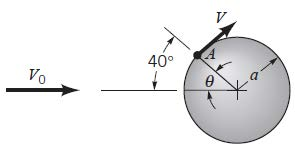
\includegraphics{Problem4.jpg}
\end{center}

\subsection*{Answer}
At $A$, the speed of fluid along the front part of the sphere is
\begin{align*}
    V_A &= \frac{3}{2} V_0 \sin{\theta_A} \\
    &= \frac{3}{2} \left(40\ \textrm{m}/\textrm{s}\right) \sin{40\degree} \\
    &= 60\sin{40\degree}\ \textrm{m}/\textrm{s}
\end{align*}
Let $\mathbf{s}$ be the unit vector in the direction of the streamwise velocity, $\mathbf{n}$ be the unit vector in the direction of the normal velocity. The velocity of the fluid at a certain point on the sphere is
\begin{equation}
    \mathbf{v} = V \mathbf{\hat{s}}
\end{equation}
Therefore, the acceleration of the fluid at that certain point is
\begin{align*}
    \mathbf{a} &= \frac{d\mathbf{v}}{dt} \\
    &= \frac{\partial \mathbf{v}}{\partial t} + \left(\mathbf{v} \cdot \nabla\right)\mathbf{v}\\
    &= V \frac{\partial \mathbf{\hat{s}}}{\partial t} + \frac{\partial V}{\partial t}\mathbf{\hat{s}} + V \frac{\partial \mathbf{v}}{\partial s} \\
    &= V \cdot \frac{V}{a} \mathbf{\hat{n}} + \mathbf{0} + V \frac{\partial \mathbf{v}}{\partial \theta} \frac{\partial \theta}{\partial s} \\
    &= \frac{V^2}{a} \mathbf{\hat{n}} + V \frac{\partial V}{\partial \theta} \cdot \frac{1}{a} \mathbf{{\hat{s}}}
\end{align*}
Therefore, our streamwise acceleration is
\begin{align*}
    a_s &= \frac{V}{a} \cdot \frac{\partial V}{\partial \theta} \\
    &= \frac{V}{a} \cdot \frac{\partial \left(\frac{3}{2}V_0 \sin{\theta}\right)}{\partial \theta} \\
    &= \frac{\frac{3}{2} V_0 \sin{\theta}}{a} \cdot \frac{3}{2} V_0 \cos{\theta} \\
    &= \frac{9}{4} \frac{{V_0}^2}{a} \sin{\theta} \cos{\theta} \\
    (a_s)_A &= \frac{9}{4} \frac{({40\ \textrm{m/s}})^2}{0.20\ \textrm{m}} \sin{40\degree} \cos{40\degree} \\
    &= 8863.270\ \textrm{m/s}
\end{align*}
and our normal acceleration is
\begin{align*}
    a_n &= \frac{V^2}{a} \\
    (a_n)_A &= \frac{\left(60 \sin{40\degree}\right)^2}{0.2\ \textrm{m}} \\
    &= 7437.166\ \textrm{m/s}
\end{align*}
\newpage

\section*{Problem 5}
Assume the temperature of the exhaust in an exhaust pipe can be approximated by $T = T_0 \left(1 + ae^{-bx}\right)\left[1 + c \cos{\omega t}\right]$, where $T_0 = 100\degree \textrm{C}$, $a = 3$, $b = 0.03 \textrm{m}^{-1}$, $c = 0.05$, and $\omega = 100\ \textrm{rad/s}$. If the exhaust speed is a constant 3 m/s, determine the time rate of change of temperature of the fluid particles at $x$ = 0 and $x$ = 4 m when $t$ = 0.

\subsection*{Answer}
As the exhaust come from a pipe, it only should move in one direction. We may determine the time rate of change of temperature of the fluid particles by using the following equation:
\begin{equation}
    \frac{DT}{Dt} = \frac{\partial T}{\partial t} + \mathbf{v} \cdot \nabla T
\end{equation}
For the first term,
\begin{align*}
    \frac{\partial T}{\partial t} &= \frac{\partial}{\partial t} \left[T_0 \left(1 + ae^{-bx}\right)\left[1 + c \cos{\omega t}\right]\right] \\
    &= T_0 \left(1 + ae^{-bx}\right)\left(-\omega c \sin{\omega t}\right) \\
\end{align*}
For the second term,
\begin{align*}
    \mathbf{v} \cdot \nabla T &= v_x \cdot \frac{\partial T}{\partial x} \\
    &= (u) \cdot T_0 \left(-abe^{-bx} \right)\left[1 + c \cos{\omega t}\right] \\
    &= -T_0 u \left(abe^{-bx} \right)\left[1 + c \cos{\omega t}\right]
\end{align*}
Therefore,
\begin{align*}
    \frac{DT}{Dt} &= T_0 \left(1 + ae^{-bx}\right)\left(-\omega c \sin{\omega t}\right) - T_0 u \left(abe^{-bx} \right)\left[1 + c \cos{\omega t}\right] \\
    &= -T_0 \left[\left(1 + ae^{-bx}\right)\left(\omega c \sin{\omega t}\right) + u \left(abe^{-bx} \right)\left[1 + c \cos{\omega t}\right]\right]
\end{align*}
Thus, for $t$ = 0 and $x$ = 0,
\begin{align*}
    \frac{DT}{dt} &= -(100 + 273.15) [(1 + 3e^{-0}) (100 \cdot 0.05 \sin{0}) + 3 \left(0.03e^{-0} \right) \left(1 + 0.05 \cos{0}\right)] \\
    &= -105.788\ \textrm{K/s}
\end{align*}
and for $x$ = 4 m,
\begin{align*}
    \frac{DT}{dt} &= -(100 + 273.15) [(1 + 3e^{-0.03 \cdot 4}) (100 \cdot 0.05 \sin{0}) + 3 \left(0.03e^{-0.03 \cdot 4} \right) \left(1 + 0.05 \cos{0}\right)] \\
    &= -93.826\ \textrm{K/s}
\end{align*}

\end{document}